%========================================
%                            Chapter                            
%======================================== 
\chapter{{\uu}: Smartphone Authentication \protect \\ Using Gestures in the Air}

In this chapter, we propose a new authentication method for smartphones. During the authentication period, the smartphone's built-in speaker transmits ultrasound signals continuously and the user draws a user-defined gesture in the air. Then the signals reflected from the user's hand are fed into a pre-trained machine learning model to get the authentication results. The key idea is to use in-phase (I) and quadrature(Q) components to represent hand movements, which not only provides high accuracy but also decrease the data size. Moreover, to calculate I/Q components, we choose to use cascaded integrator–comb (CIC) filters, which utilizes only delay and addition and subtraction. Since CIC filters require no multiplication operations, it does not introduce high computational overhead and therefore can be implemented on most smartphones. Experiments of the proposed {\uu} system on Google Nexus 6P devices show that the system can identify 3 different gestures with an average accuracy of 90.89\% and identify 6 people with an average accuracy of 78.47\%. We also propose six directions to further increase the accuracy, as a guide for future work.


%========================================
%                            Section                             
%======================================== 	 
\section{Introduction}
Smartphones have been an indispensable part of our daily lives, and most of them still require a password or pin code if you want to unlock them. However, in today’s busy world, typing those passwords is a waste of time. As a result, biometric security systems have been on the rise and many smartphones adopt the fingerprints to do authentication. The problem is, if your hands are dirty or wet, the smartphone just won’t let you in! Researchers have developed a lot more other authentication methods, such as the face ID or smart card, but these methods all require special hardware. Moreover, if users wear face masks, air-purifying respirators, goggles, or face shields, as during the COVID-19 pandemic, authentication methods such as face ID do not work anymore. Some may argue that users can use voice authentication systems instead. However, the security of voice authentication systems is relatively low due to the replay attack and many users don't use the method in public because it’s uncomfortable talking to their phones with others around.

Therefore, we propose a new authentication method called {\uu}, which provides a silent, quick, and smooth user experience for unlocking without your hands touch the phone. It utilizes the speakers and microphones and conducts the authentication through processing ultrasound signals. The smartphone has the ability to reconstruct the user’s hand movement and determine whether it belongs to a legitimate user or not. Following the classification method proposed in~\cite{vongsingthong2015survey}, our method is a combination of knowledge-based method and identity-based method, since the user must have the knowledge of what the shape he should draw and meet the biometric features of how to draw the shape.

%========================================
%                            Section                             
%======================================== 	 
\section{Related Works}
Our {\uu} system has three important building blocks: 1) smartphones can generate and process ultrasound signals 2) the ultrasound signals are sensitive to hand movements 3) hand movements are feasible features for user authentication. There have been many researches on each  building block.

First, commercial on-the-shelf smartphones can transmit and receive ultrasound signals, though the band is very narrow. Smartphones nowadays are mostly equipped with speakers and microphones whose highest sample rate is either 44100 Hz or 48000 Hz~\footnote{Some models support higher resolution, for example, Samsung Galaxy S10 features 32-bit/384kHz Hi-Fi playback}. According to NyquistShannon sampling theorem, in order to sample a signal of frequency $f$, a sufficient sample rate would be $2f$. Then by the reverse, we know that commercial smartphones can generate and record sounds whose frequency are lower than 22050 Hz or 24000 Hz. Since, the range of human hearing is generally considered to be 20 Hz - 20000 Hz, we conclude that smartphone are able to create and process ultrasounds in the range of 20000 Hz - 22050 Hz or 20000 Hz - 24000 Hz.

Next, various algorithms have been developed to extract information of movements from ultrasound signals.  Graham et al.~\cite{graham2015software} proposed a smartphone sonar system which calculates distances by measuring the elapsed time between the initial pulse of ultrasound signal and its reflection. They were able to measure the distances of objects accurately with an error bound of 12 cm. Liu et al.~\cite{liu2015guoguo} designed the Guoguo algorithm and ecosystem to realize the smartphone-based fined-grained indoor localization with average localization accuracy being about 6 cm - 15 cm in typical indoor environments. Nandakumar et al.~\cite{nandakumar2016fingerio} presented a sub-centimeter level smartphone tracking system which adopts a modulation technique commonly used in wireless communication called orthogonal frequency division multiplexing. Their FingerIO system can achieve 2D finger tracking with an average accuracy of 8 mm. Mao et al.~\cite{mao2016cat} developed a high-precision acoustic tracker system by sending a distributed frequency
modulated continuous waveform (FMCW). They also designed an optimization framework which combines FMCW estimation with Doppler shifts and inertial measurement unit measurements to enhance the accuracy to be 8 mm - 9 mm in 3D space. Wang et al.~\cite{wang2016device} proposed LLAP system which measures the phase changes of the sound signals caused by hand/finger movements and then converts the phase changes into the distance of the movement. They increase the tracking accuracy to 7 mm in 2D space. Later on, Yun et al.~\cite{yun2017strata}  took into account multi-path propagation, and designed a novel acoustic based device-free tracking system, called Strata, which outperforms FingerIO and LLAP. In 2018, Sun et al.~\cite{sun2018vskin} improved LLAP and  the new system can capture finger movements with an accuracy of 3.59 mm. 

Lastly, hand movements have intra-person similarity and inter-person difference. Therefore, it can be used for user authentication. There have been many finger/hand movement based authentication methods literatures. Niu et al.~\cite{niu2011gesture} proposed using finger gestures with taps to the screen to conduct authentication. They tested the recall and forgery of gesture authentication and show, using dynamic time warping, that even simple gestures are repeatable by their creators yet hard to forge by attackers when taps are added. Hong et al.~\cite{hong2015waving} proposed Waving Authentication (WA) which is a motion gesture authentication system based on accelerometers. WA utilizes eight distinguishing features hiding in the acceleration traces of motion gestures and exploits one-class Support Vector Machine for classification. Yang et al.~\cite{yang2016free} studied how free-form gestures perform in the wild. Their 91 participants generated 347 text passwords and 345 gesture passwords with 2002 completed log-in tasks. They found that, with gesture passwords, participants generated new passwords and authenticated faster with comparable memorability while being more willing to retry. 

However, all the above gestures are collected from the smartphone touch screens. There is no existing paper on how to authenticate users based on their hand movements in the air.

%========================================
%                            Section                             
%======================================== 
\section{Background}\label{sec:handIQ}
The general idea of {\uu} is to treat hand movements as a special I/Q modulation on a signal with fixed frequency. Different users have different hand movements, and modulate the same carrier signal in different ways. After collecting the modulated signals, machine learning techniques can be used for modulation classification. If the modulation is classified to be the hand movement of a legitimate user, the smartphone will accept that user. 

In this section, we first provides necessary background on I/Q data, and then discuss the relationship between hand movements and I/Q modulation.

\subsection{I/Q components and I/Q modulation}
\begin{figure}[!h]
	\centering
	\includegraphics[width=.8\linewidth]{iqdata1}
	\begin{minipage}{.4\linewidth}
		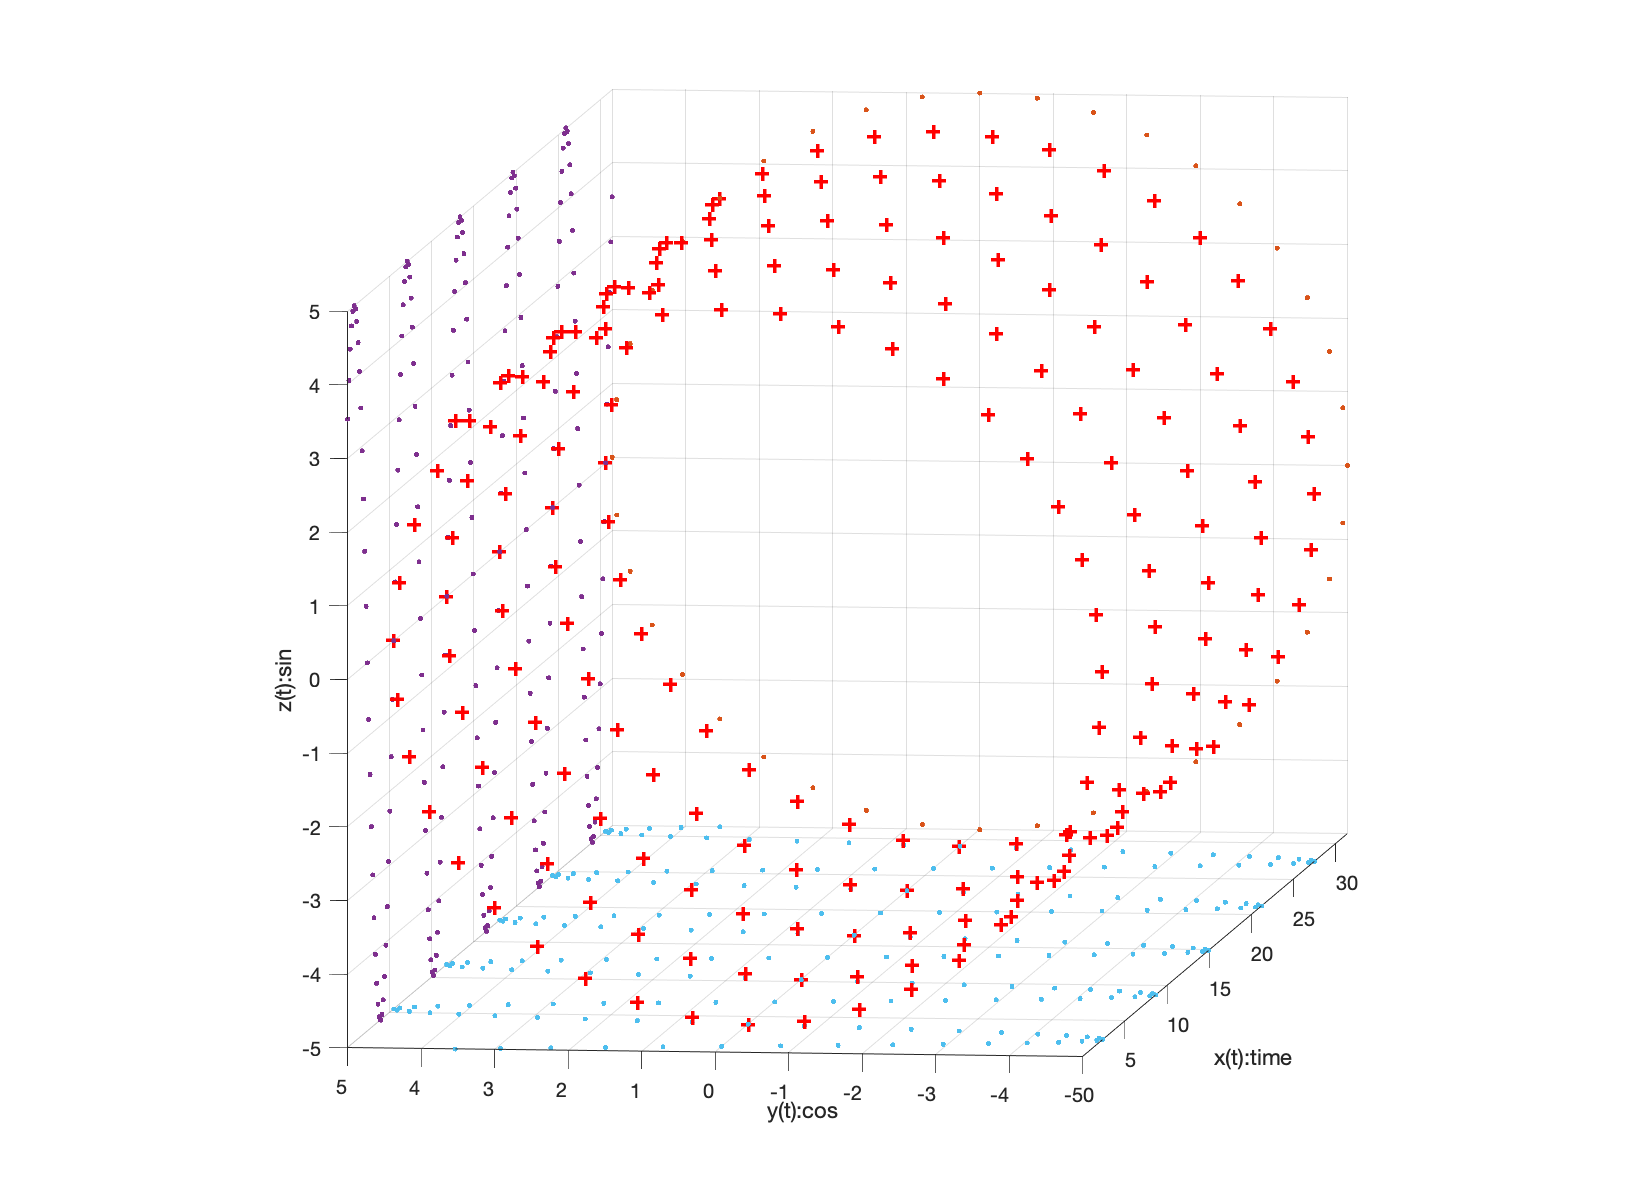
\includegraphics[width=\linewidth]{iqdata2}
	\end{minipage}
	\hfil
	\begin{minipage}{.5\linewidth}
		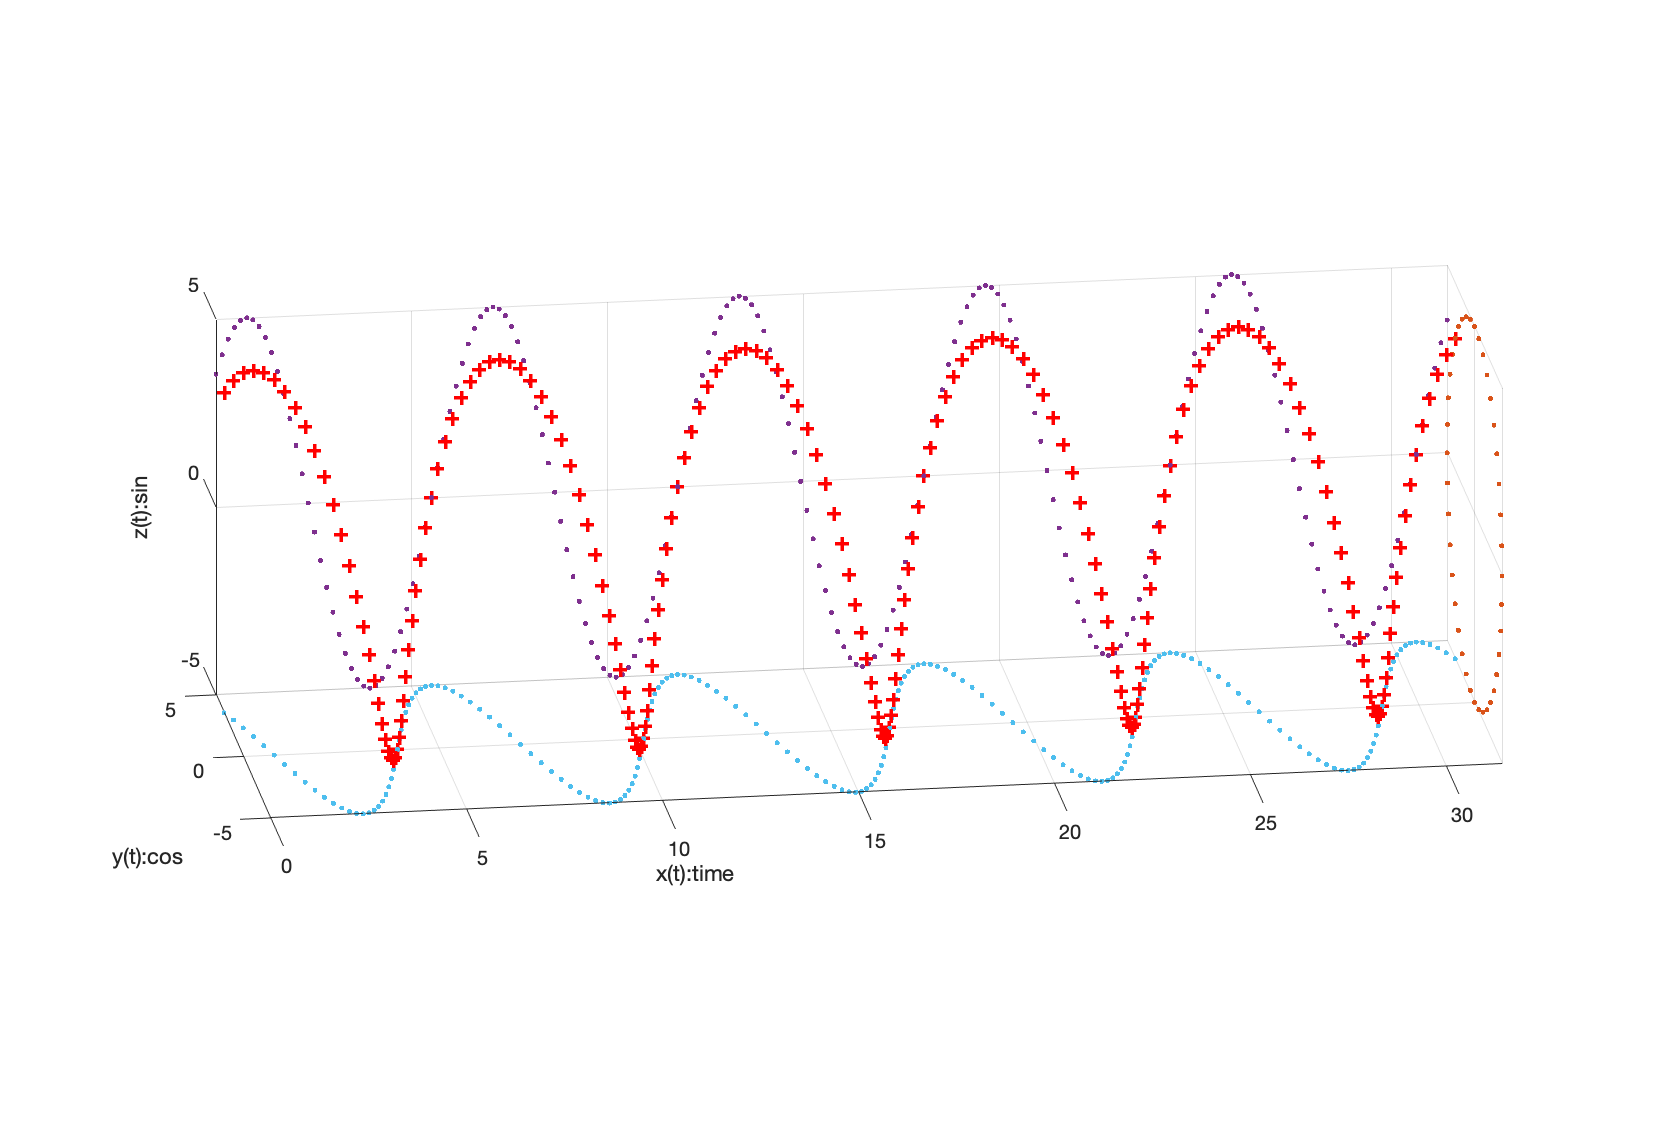
\includegraphics[width=\linewidth]{iqdata3}
		\includegraphics[width=\linewidth]{iqdata4}
	\end{minipage}
	\caption{In-phase and Quadrature Components from Different View Angles}
	\label{fig:iqdata}
\end{figure}

The most common way to represent a wave is to use a series of samples of the momentary amplitude of the signal. However, this method cannot differentiate between a positive or negative frequency since they both generate the same curve, for example,  $\cos(x) = \cos(-x)$. This becomes a problem working with the signal. Mixing (multiplying) two signals and it'll cause multiple solutions due to the uncertainty of the sign. A better way is using I/Q data and representing a wave using in-phase and quadrature components. As shown in Figure~\ref{fig:iqdata}, the signal is plotted in three dimensions. The in-phase component and the quadrature component are the 2D projections of the signal. I/Q data together show the changes in amplitude and phase of a sine wave. The in-phase component indicates the ``real'' signal. For two signals of a positive and a negative frequency, they will have the same in-phase component but reversed quadrature components. Moreover, if the signal is viewed along the time axis, the spiral winds counter-clockwise, which means the frequency is positive. The radius of each circle indicates the peak amplitude of the signal.

Mathematically, for a complex signal $Ae^{i \varphi }$ where $i$ is the imaginary unit, the in-phase component is $I = A\cos(\varphi)$ and the quadrature component is $Q = A\sin(\varphi)$. That is,
\begin{displaymath}
	Ae^{i \varphi } = A \cdot (\cos(\varphi) + i \cdot \sin(\varphi)) = I + Qi
\end{displaymath}
\begin{displaymath}
 A = \sqrt{I^2 + Q^2}  \quad \text{and} \quad \varphi = \tan^{-1}\frac{Q}{I}
\end{displaymath}


In electrical engineering, there are three basic ways to modulate a waveform: Amplitude Modulation (AM), Frequency Modulation (FM) and Phase Modulation (PM). All of them can be achieved by I/Q modulation. Suppose the carrier's frequency is $f$, I/Q modulation is to solve the following equation:
\begin{displaymath}
\texttt{ModulatedSignal} = I \cdot \cos(2 \pi f t) + Q \cdot \sin(2 \pi f t) .
\end{displaymath}
To decode the baseband signal, signal multiplication and low pass filters are needed:
\begin{align*}
I =~&\texttt{lowpass} (\texttt{ModulatedSignal}  \cdot  \cos(2 \pi f t) ) ;\\        
Q=~&\texttt{lowpass} (\texttt{ModulatedSignal}  \cdot \sin(2 \pi f t) ) .
\end{align*}

\subsection{Hand Movements and I/Q Data}
Now we show how hand movements can be regarded as I/Q modulation. As shown in Figure~\ref{fig:soundpath}, the smartphone speaker plays an ultrasound signal $A\cos \left (2\pi f \frac{n}{f_s}\right)$ with the peak amplitude of $A=1$, the frequency $f = 20,000 $~Hz, and the sampling frequency of $f_s = 44,100 $~Hz. At the time $t_p = \frac{n}{f_s}$, the sound propagation path $p$ decreases by $\Delta p$ due to the hand movement. The received signal therefore becomes $2A^\prime_p \cos \left (2\pi f \frac{n}{f_s}  - 2 \pi \frac{\Delta p}{\lambda} - \theta p\right)$, where $2A^\prime_p$ is the new amplitude, the term $2 \pi \frac{\Delta p}{\lambda}$ comes from the phase lag caused by the propagation delay of $\frac{\Delta p}{\lambda}$ and $\lambda$ is the wavelength of the ultrasound. In our system, $\lambda = c/f = \frac{343 \text{~m/s}}{20,000 \text{~Hz}} = 1.72 \text{~cm}$, where $c$ is the speed of sound. The last term $ \theta p$ is the  initial phase, which is caused by the hardware delay and phase inversion due to reflection~\cite{wang2016device}.  
In conclusion, the existence of hand movement changes the amplitude and phase of the original signal. Since I/Q data shows the changes in amplitude and phase of a waveform, we use I/Q data to represent hand movements.

\begin{figure}[h]
	\centering
	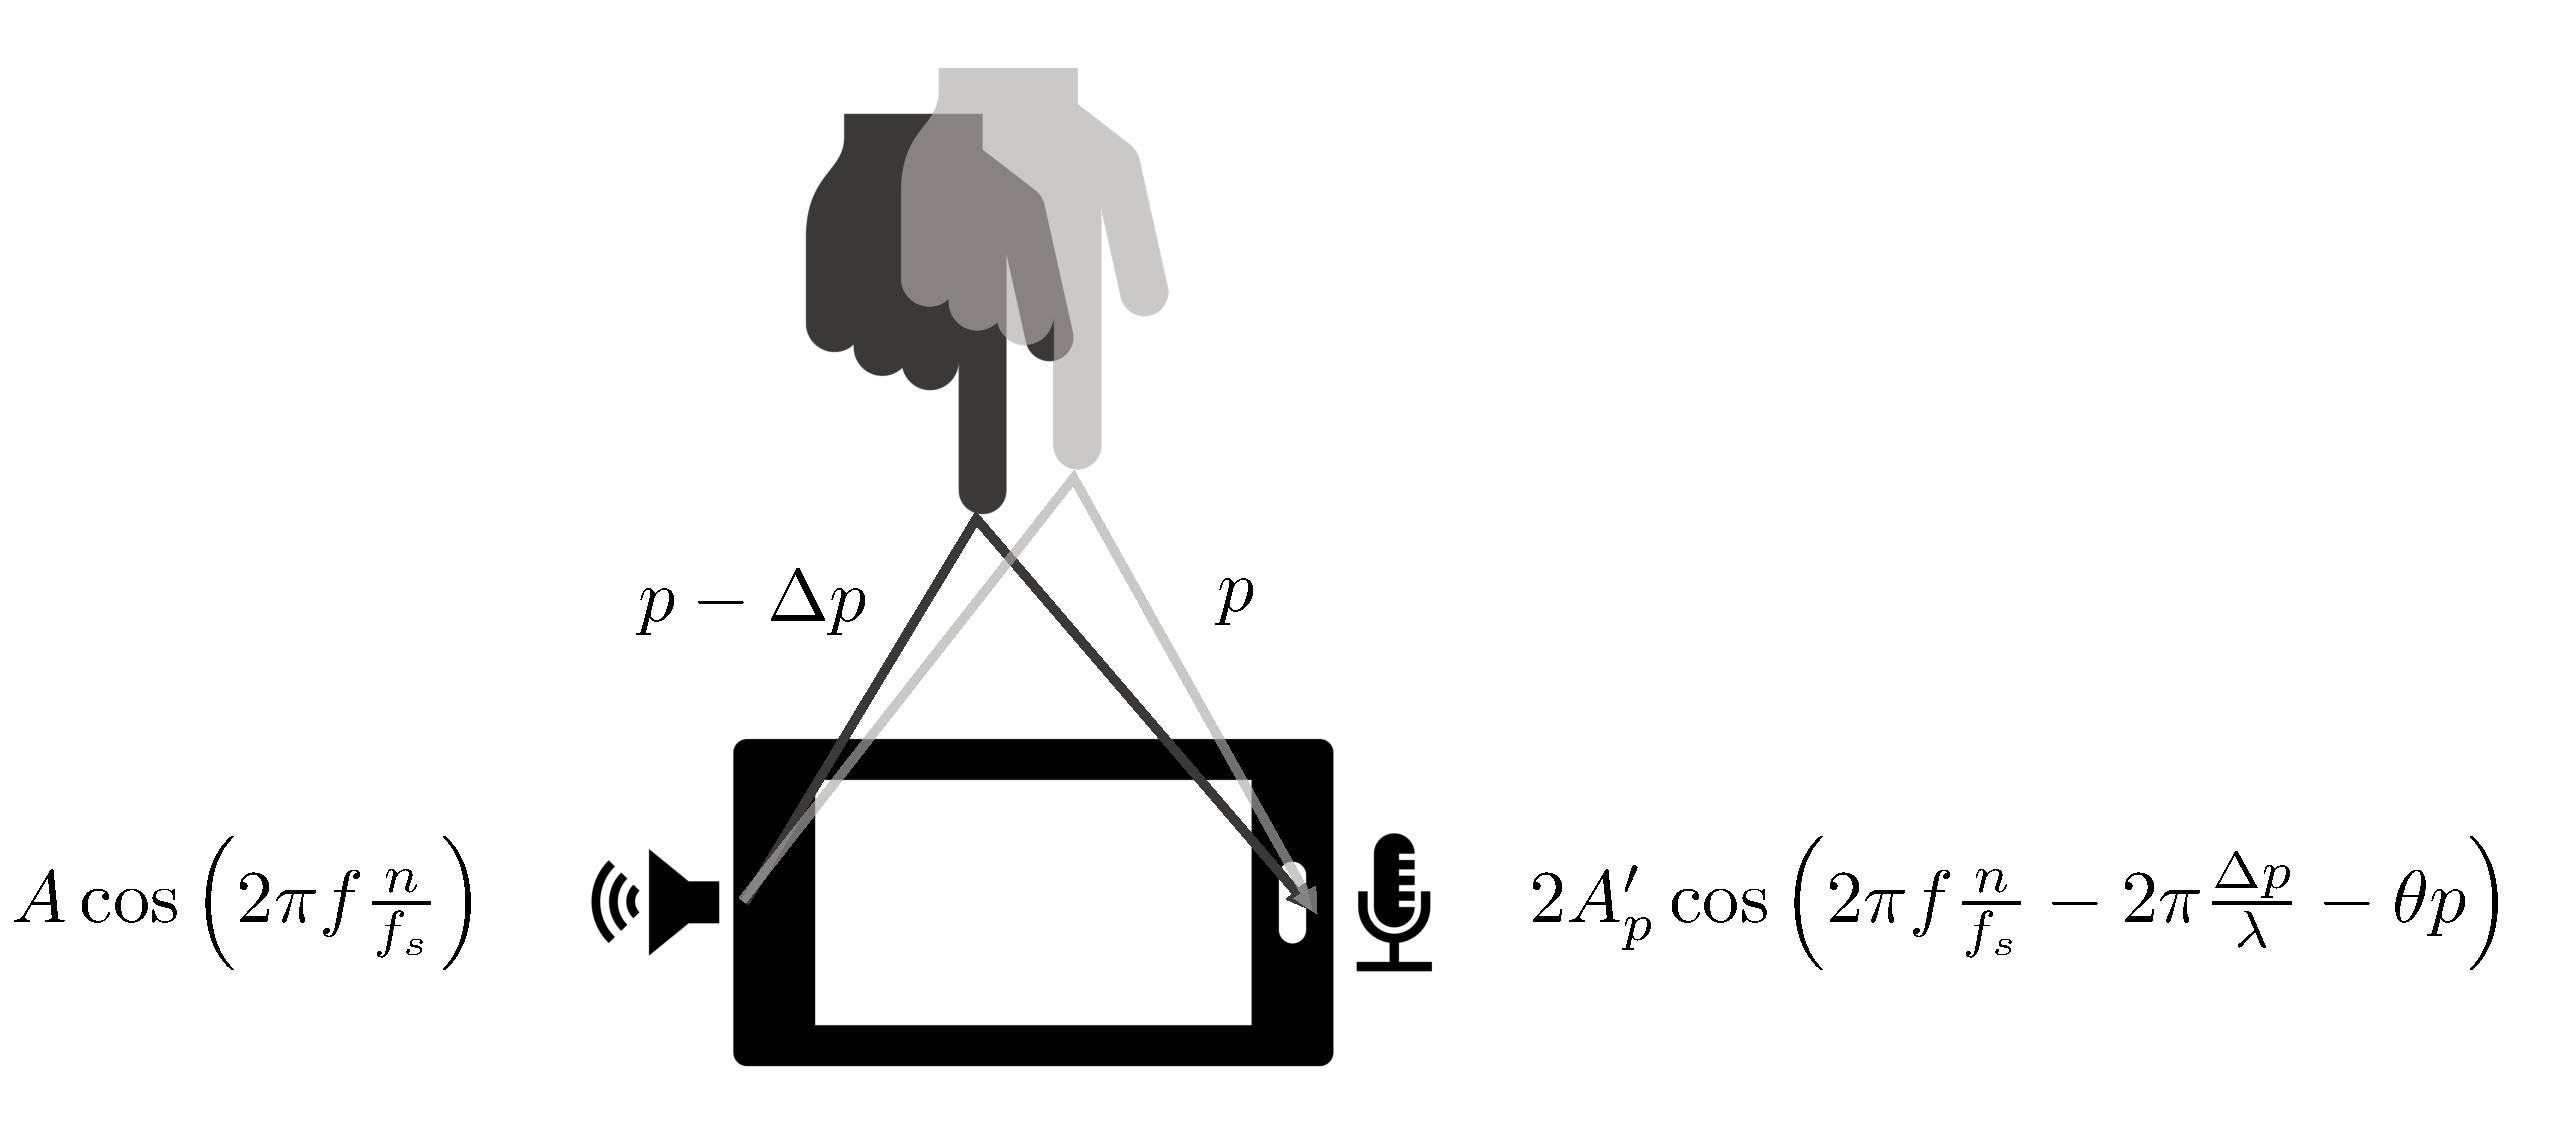
\includegraphics[width=.8\linewidth]{path}
	\caption{Sound Propagation Paths on a Smartphone.}
	\label{fig:soundpath}
\end{figure}

To calculate the in-phase value, we first multiply the received signal by $\cos \left (2\pi f \frac{n}{f_s}\right)$:
\begin{align*}
&2A^\prime_p \cos \left (2\pi f \frac{n}{f_s}  - 2 \pi \frac{\Delta p}{\lambda} - \theta p\right) \times \cos \left (2\pi f \frac{n}{f_s}\right)\\        
=~&A^\prime_p \cos \left (2\pi f \frac{n}{f_s}  - 2 \pi \frac{\Delta p}{\lambda} - \theta p - 2\pi f \frac{n}{f_s}\right)  + A^\prime_p \cos \left (2\pi f \frac{n}{f_s}  - 2 \pi \frac{\Delta p}{\lambda} - \theta p + 2\pi f \frac{n}{f_s}\right)  \\
=~&A^\prime_p \cos \left( - 2 \pi \frac{\Delta p}{\lambda} - \theta p \right)  + A^\prime_p \cos (4\pi f \frac{n}{f_s}  - 2 \pi \frac{\Delta p}{\lambda} - \theta p )  .
\end{align*}

Note that the second term $A^\prime_p \cos \left(4\pi f \frac{n}{f_s}  - 2 \pi \frac{\Delta p}{\lambda} - \theta p \right) $ is a signal of frequency $2f$ and will be removed after applying the low pass filter. Therefore, we get 
\begin{displaymath}
I_p = A^\prime_p \cos \left( - 2 \pi \frac{\Delta p}{\lambda} - \theta p \right) .
\end{displaymath}

Similarly, we can get the quadrature value by multiplying $-\sin \left (2\pi f \frac{n}{f_s}\right)$:
\begin{align*}
&2A^\prime_p \cos \left (2\pi f \frac{n}{f_s}  - 2 \pi \frac{\Delta p}{\lambda} - \theta p\right) \times \left(- \sin \left (2\pi f \frac{n}{f_s}\right)\right)\\        
=~&A^\prime_p \sin \left (2\pi f \frac{n}{f_s}  - 2 \pi \frac{\Delta p}{\lambda} - \theta p - 2\pi f \frac{n}{f_s}\right)  - A^\prime_p \sin \left (2\pi f \frac{n}{f_s}  - 2 \pi \frac{\Delta p}{\lambda} - \theta p + 2\pi f \frac{n}{f_s}\right)  \\
=~&A^\prime_p \sin \left( - 2 \pi \frac{\Delta p}{\lambda} - \theta p \right)  -  A^\prime_p \sin \left(4\pi f \frac{n}{f_s}  - 2 \pi \frac{\Delta p}{\lambda} - \theta p \right)   .
\end{align*}
After low pass filter, we get:
\begin{displaymath}
Q_p = A^\prime_p \sin \left( - 2 \pi \frac{\Delta p}{\lambda} - \theta p \right) .
\end{displaymath}


Combining these two components as the real and imaginary part of a complex signal, we have the complex baseband as follows: 
\begin{displaymath}
\texttt{BasebandSignal} = A^\prime_p e^{-i \left(2 \pi \frac{\Delta p}{\lambda} + \theta p\right)}.
\end{displaymath}

Note that the phase for path $p$ is $\varphi_p = \left(2 \pi \frac{\Delta p}{\lambda} + \theta p\right)$, which changes by $2\pi$ when $\Delta p$ changes by the amount of sound wavelength $\lambda = 1.72 \text{~cm}$. In other words, a small
movement of a few millimeters will significantly change the phase of the received sound wave. 

In conclusion, if there is no hand movement at the time $t_p$, i.e., $\Delta p = 0$,  then $I_p$ and $Q_p$ will be stable. Otherwise, the I/Q components vary like sinusoids.


%========================================
%                            Section                             
%======================================== 	 
\section{System Design}
We now provide the system design of {\uu}. The system is built based on Android operating system and tested by Google Nexus 6P smartphones.

In {\uu}, the smartphone speaker would send continuous ultrasound waves with frequency $f = 20,000 $~Hz. The signals are encoded with 16 bit pulse-code modulation (PCM). Then we use the smartphone microphones to catch the reflective signals of the ultrasound simultaneously. Though the smartphone has more than one microphones to support stereo recording, our system only need one channel to calculate the I/Q data.  As shown in Figure~\ref{fig:ultraunlockapp}, we first normalize the signal, then multiply the received signal with $\cos \left (2\pi f \frac{n}{f_s}\right)$ and $-\sin \left (2\pi f \frac{n}{f_s}\right)$. After converting the data to fixed-point data type with 16 word length and 15 fraction length, we feed the data through Cascaded Integrator-Comb (CIC) filters to remove high frequency components and decimate the signal. To achieve better computational efficiency, we do not use a frequency compensate FIR filter after the CIC but directly output the in-phase and quadrature values.



\begin{landscape}
	\begin{figure}[h]
		\centering
		\vspace{-1.7in}
		\includegraphics[width=\linewidth]{UltraUnlockApp}
		\vspace{-1.5in}
		\caption{Android App design for {\uu}}
		\label{fig:ultraunlockapp}
	\end{figure}
\end{landscape}



CIC filter is an optimized class of finite impulse response (FIR) filter combined with an decimator. It provides linear phase response and 
utilizing only delay and addition and subtraction. In other words, it requires no multiplication operations and therefore has less computational costs, which is more suitable to be implemented on smartphones.
%
Our CIC filter is a two section filter (two integrator sand two comb filters)with the decimate ratio of 15 and differential delay of 16. Figure~\ref{fig:CICFilter} shows the frequency response of the CIC filter. We select the parameters so that the first and second zeros of the filter appear at 183 Hz and 366 Hz. The pass-band of the CIC filter is 0 - 100 Hz, which corresponds to the movements with a speed lower than 0.86 m/s when the wavelength is 1.72 cm. 

\begin{figure}[h]
	\centering
	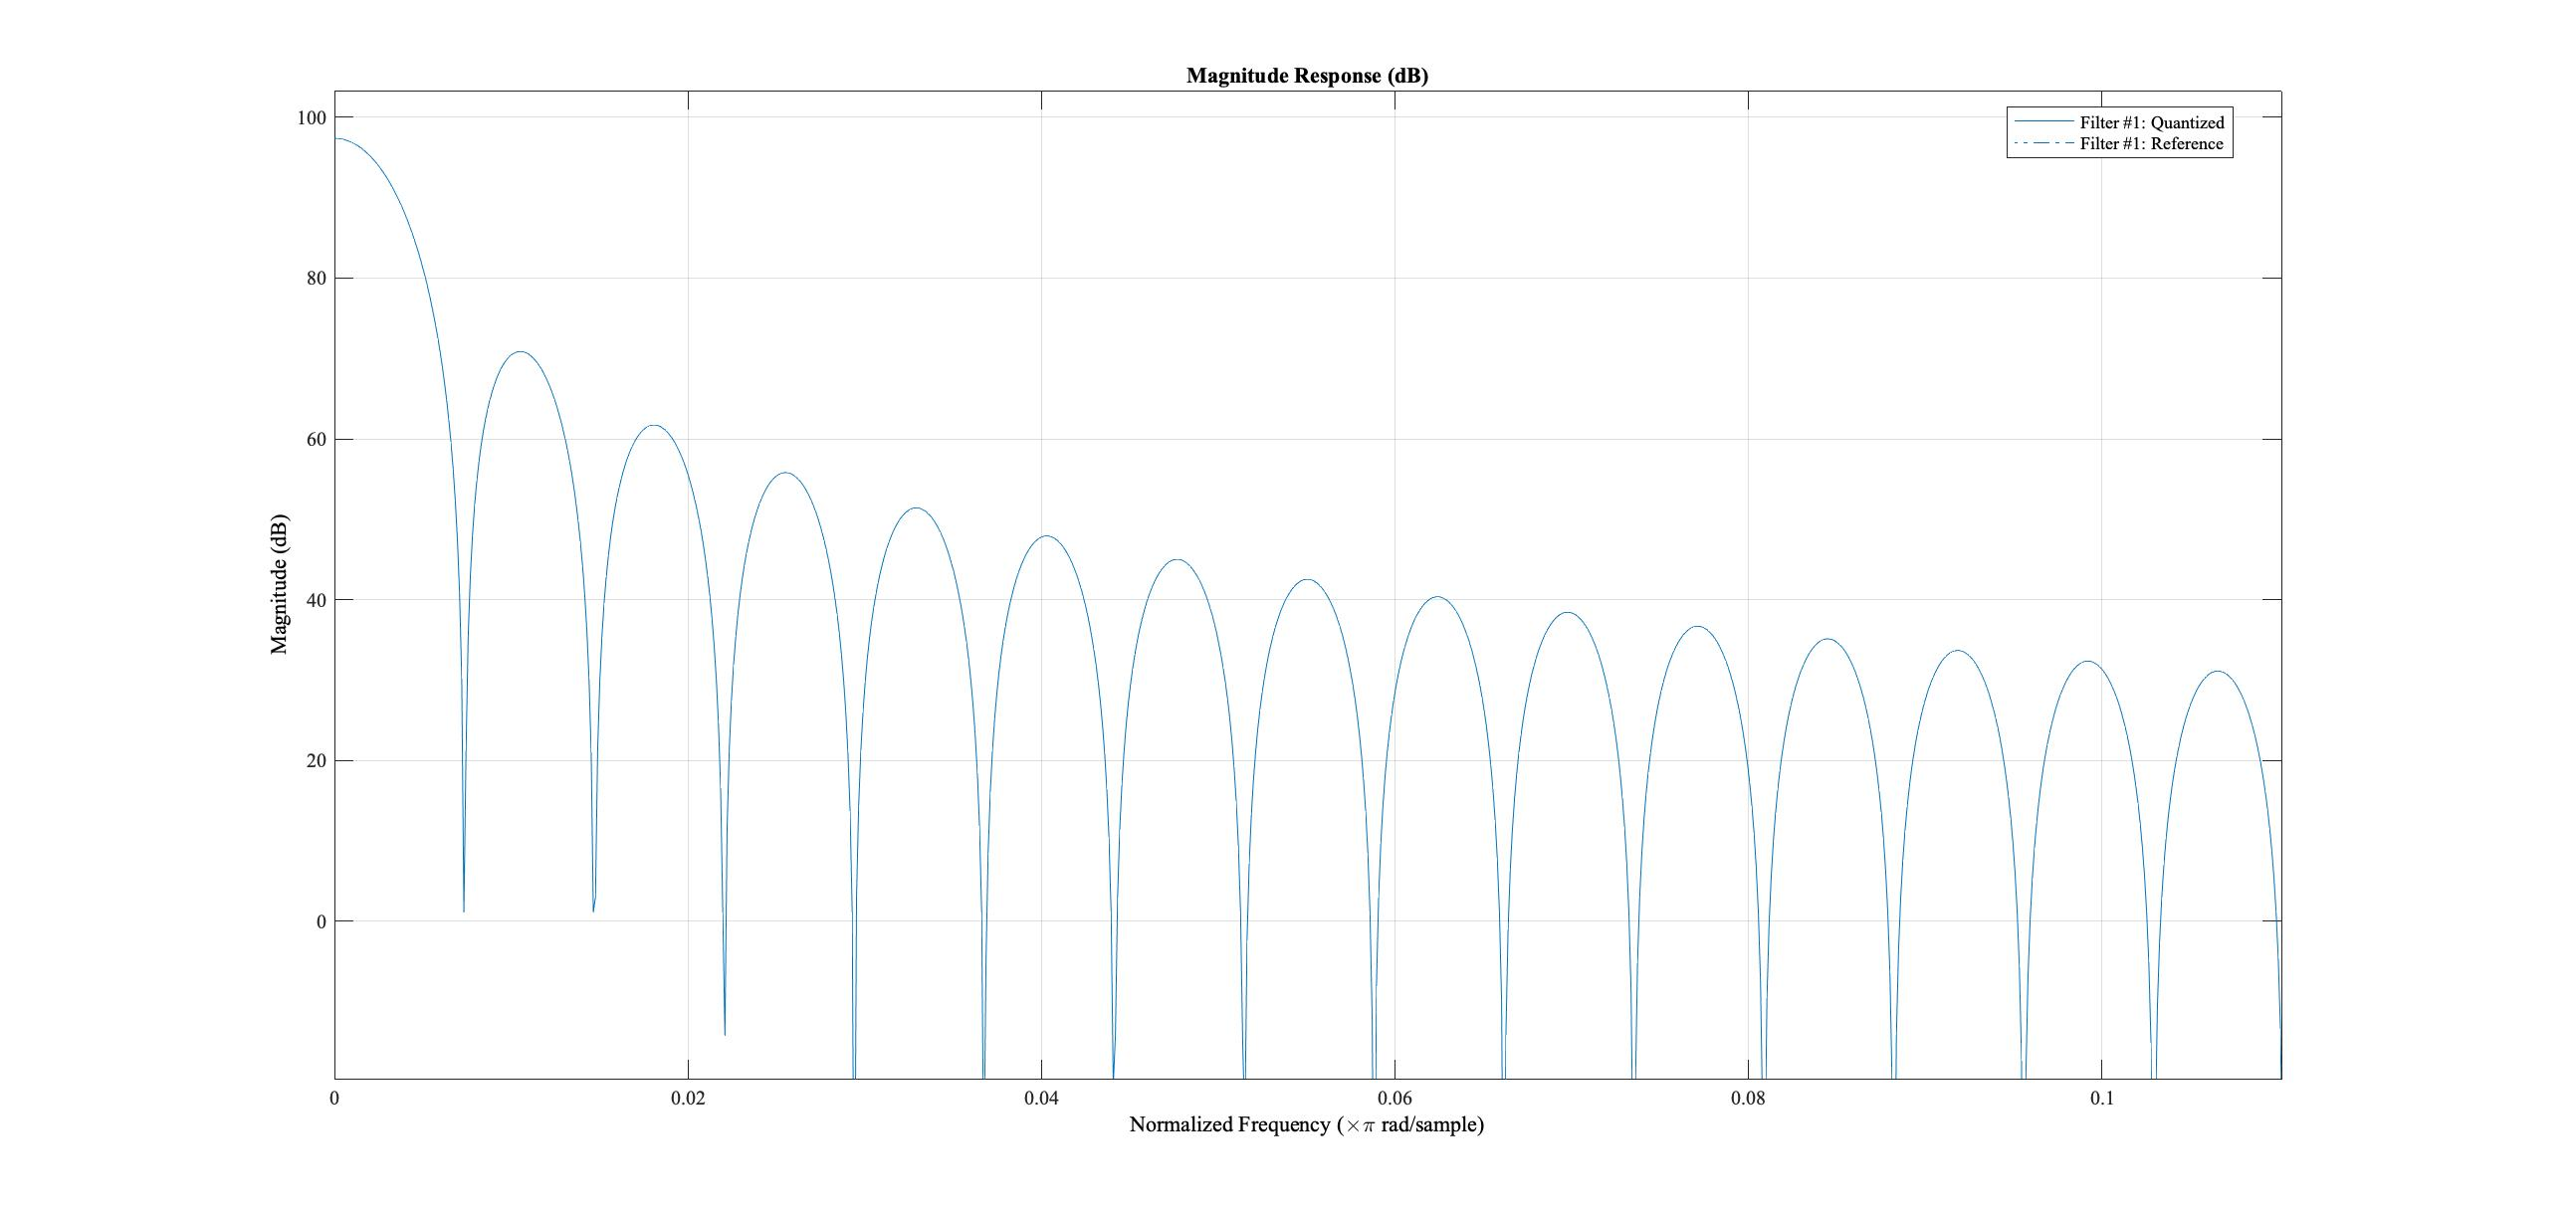
\includegraphics[width=.9\linewidth]{CICFilter}
	\caption{Frequency Response of the Cascaded Integrator-Comb Filter}
	\label{fig:CICFilter}
\end{figure}

As discussed in Section~\ref{sec:handIQ}, the in-phase and quadrature components are a good indicator of the path changes. In detail, the I/Q waveforms remain static when the hand is not moving and vary like sinusoids when the hand moves. Different hand movements generate different sinusoids, which can be trained by a Long Short-Term Memory LSTM network for classification.  We use the same LSTM network as discussed in Section~\ref{sec:LSTM}, but with different parameter settings.

%========================================
%                            Section                             
%======================================== 	 
\section{Experiment Results}

We implemented the {\uu} on a Google Nexus 6P smartphone and first validate the correlation between hand movements and I/Q data.
Three screenshots are shown in Figure~\ref{fig:realIQ}. The yellow lines are the quadrature components and the blue lines are the in-phase components. The x-axis is the indexes of samples. In each figure, 256 samples are shown, which spans in the time period of $256/294\times4410/44100 = 0.087$ s. (256 is the buffer size of the array plot, 294 is the sampling rate after CIC filter, 4410 is the frame size of audio recorder, and 44100 is the sampling frequency of the carrier signal.) As shown in Figure~\ref{fig:realIQ}, when there is no hand movement, the I/Q data are stable. When user put one hand parallel to the phone and move towards the screen, then I/Q value become regular sinusoids. If the user conduct an open-close gesture (make a loose fist and then spread all fingers wide), the I/Q data are still sinusoidal but they become less regular. Note that these screen shots cannot represent the whole changes caused by hand movement, since a whole gesture usually costs about 0.3-1 second, which spans 3 to 12 frames.


\begin{figure}[h]
	\centering
	\begin{minipage}{.6\linewidth}
		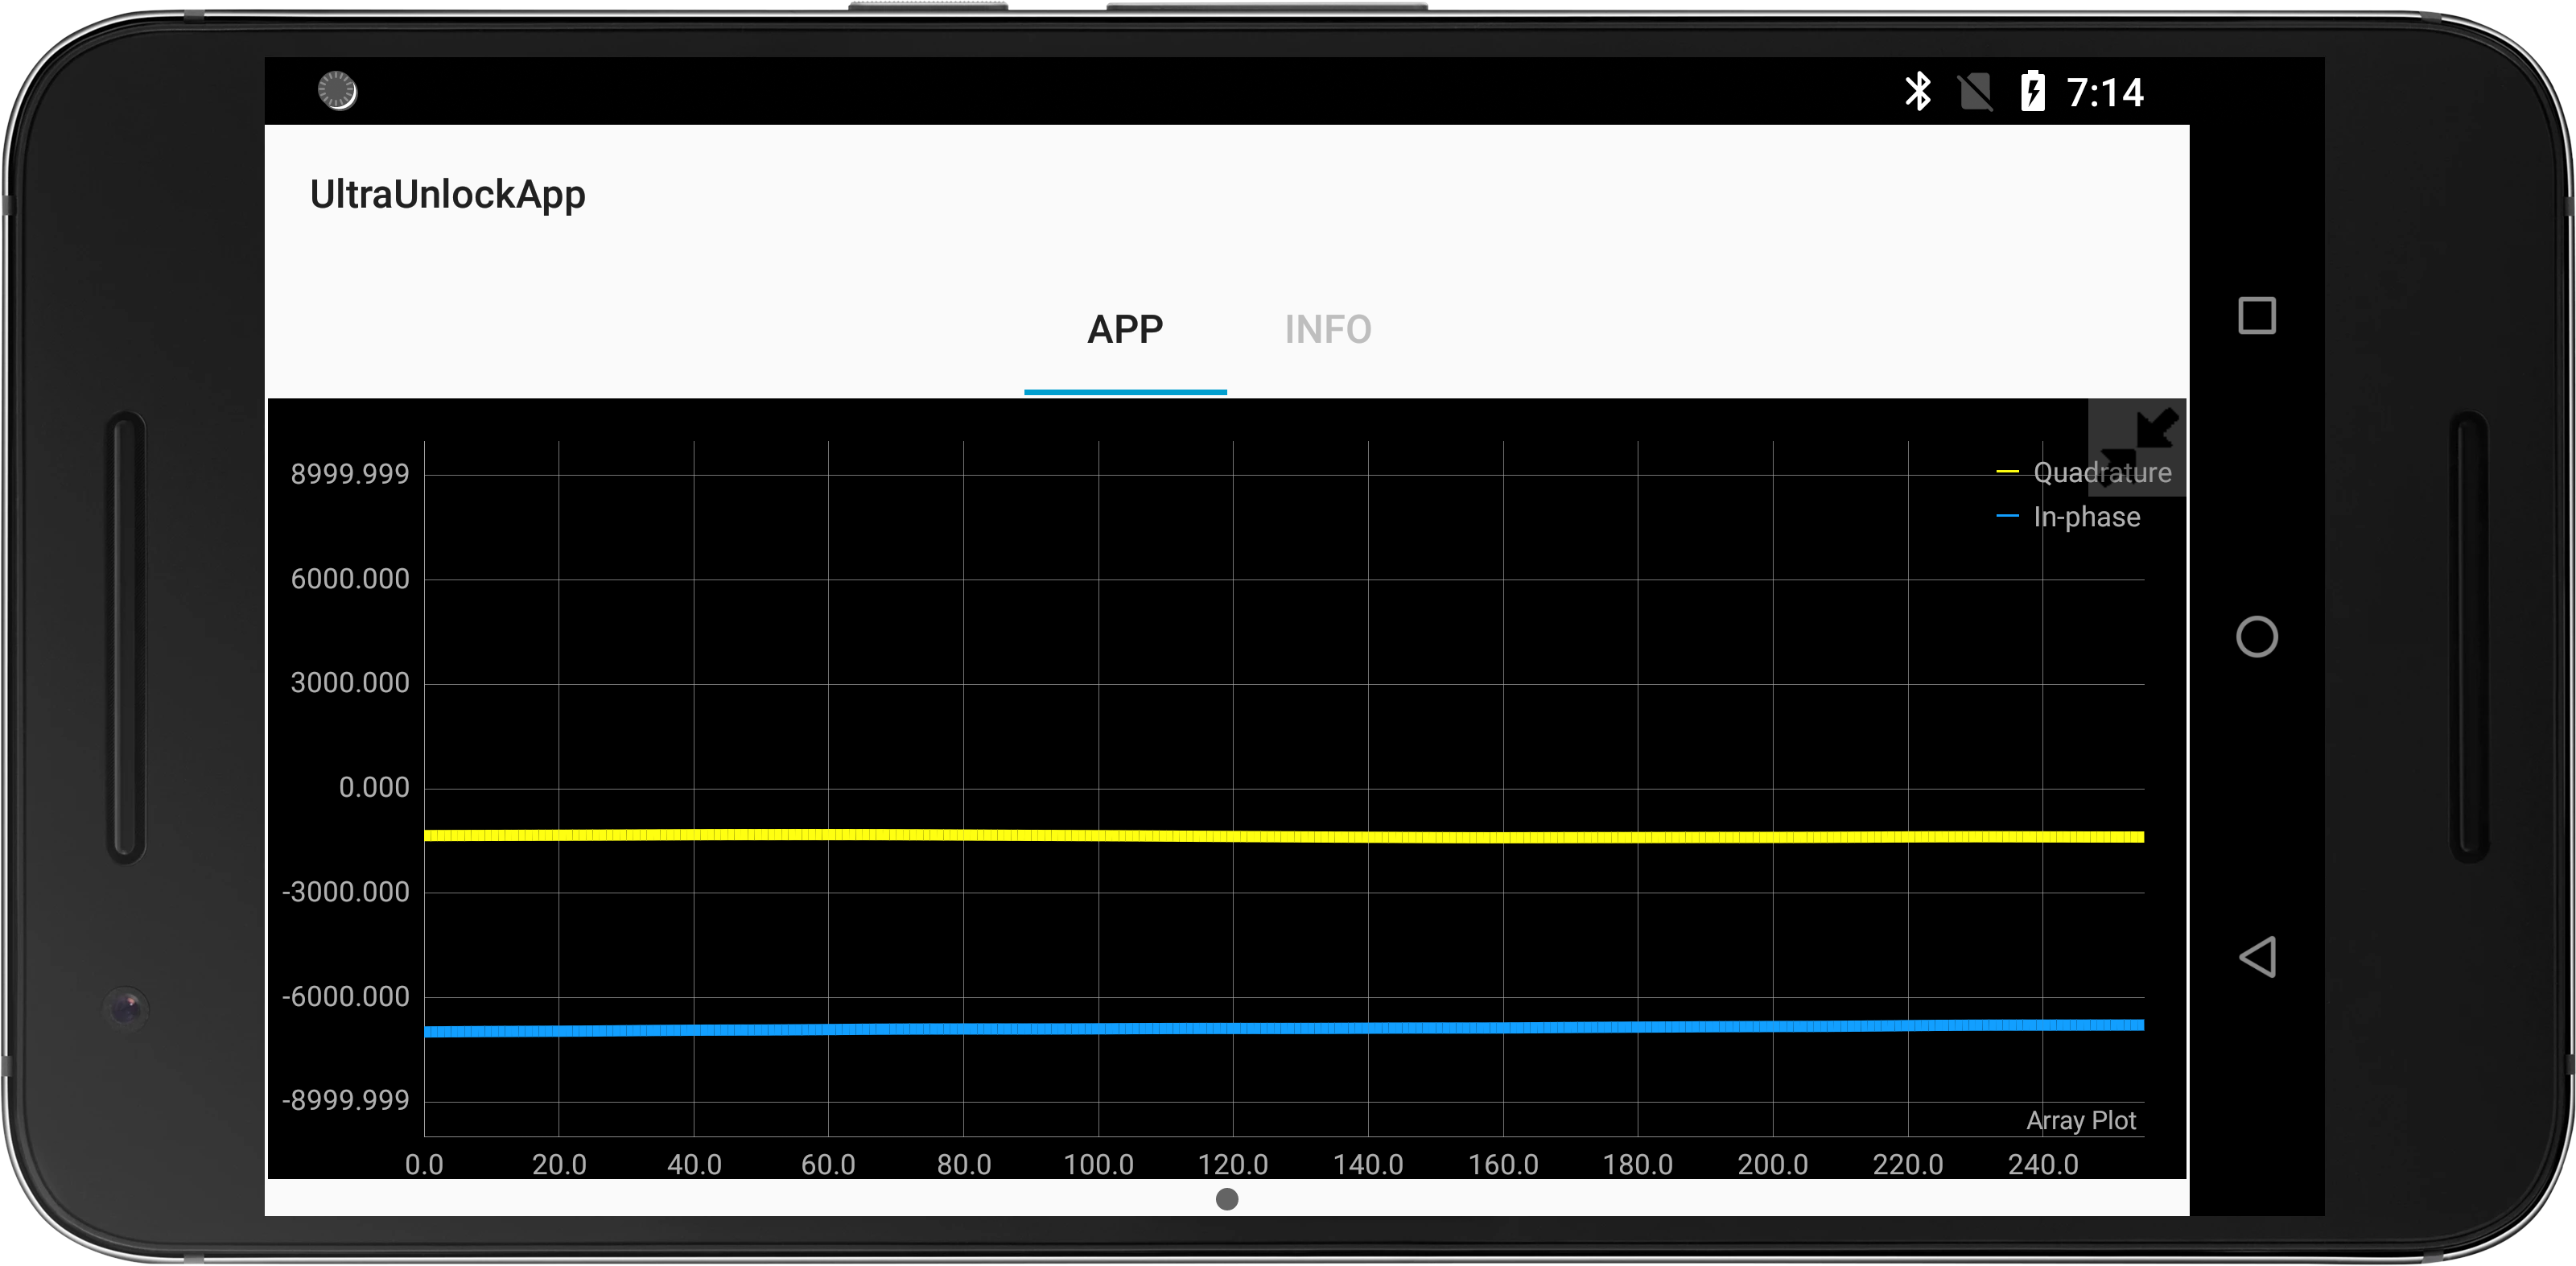
\includegraphics[width=\linewidth]{realiqdata0}
		\subcaption{No Hand Movement}
		\vspace{.1in}
		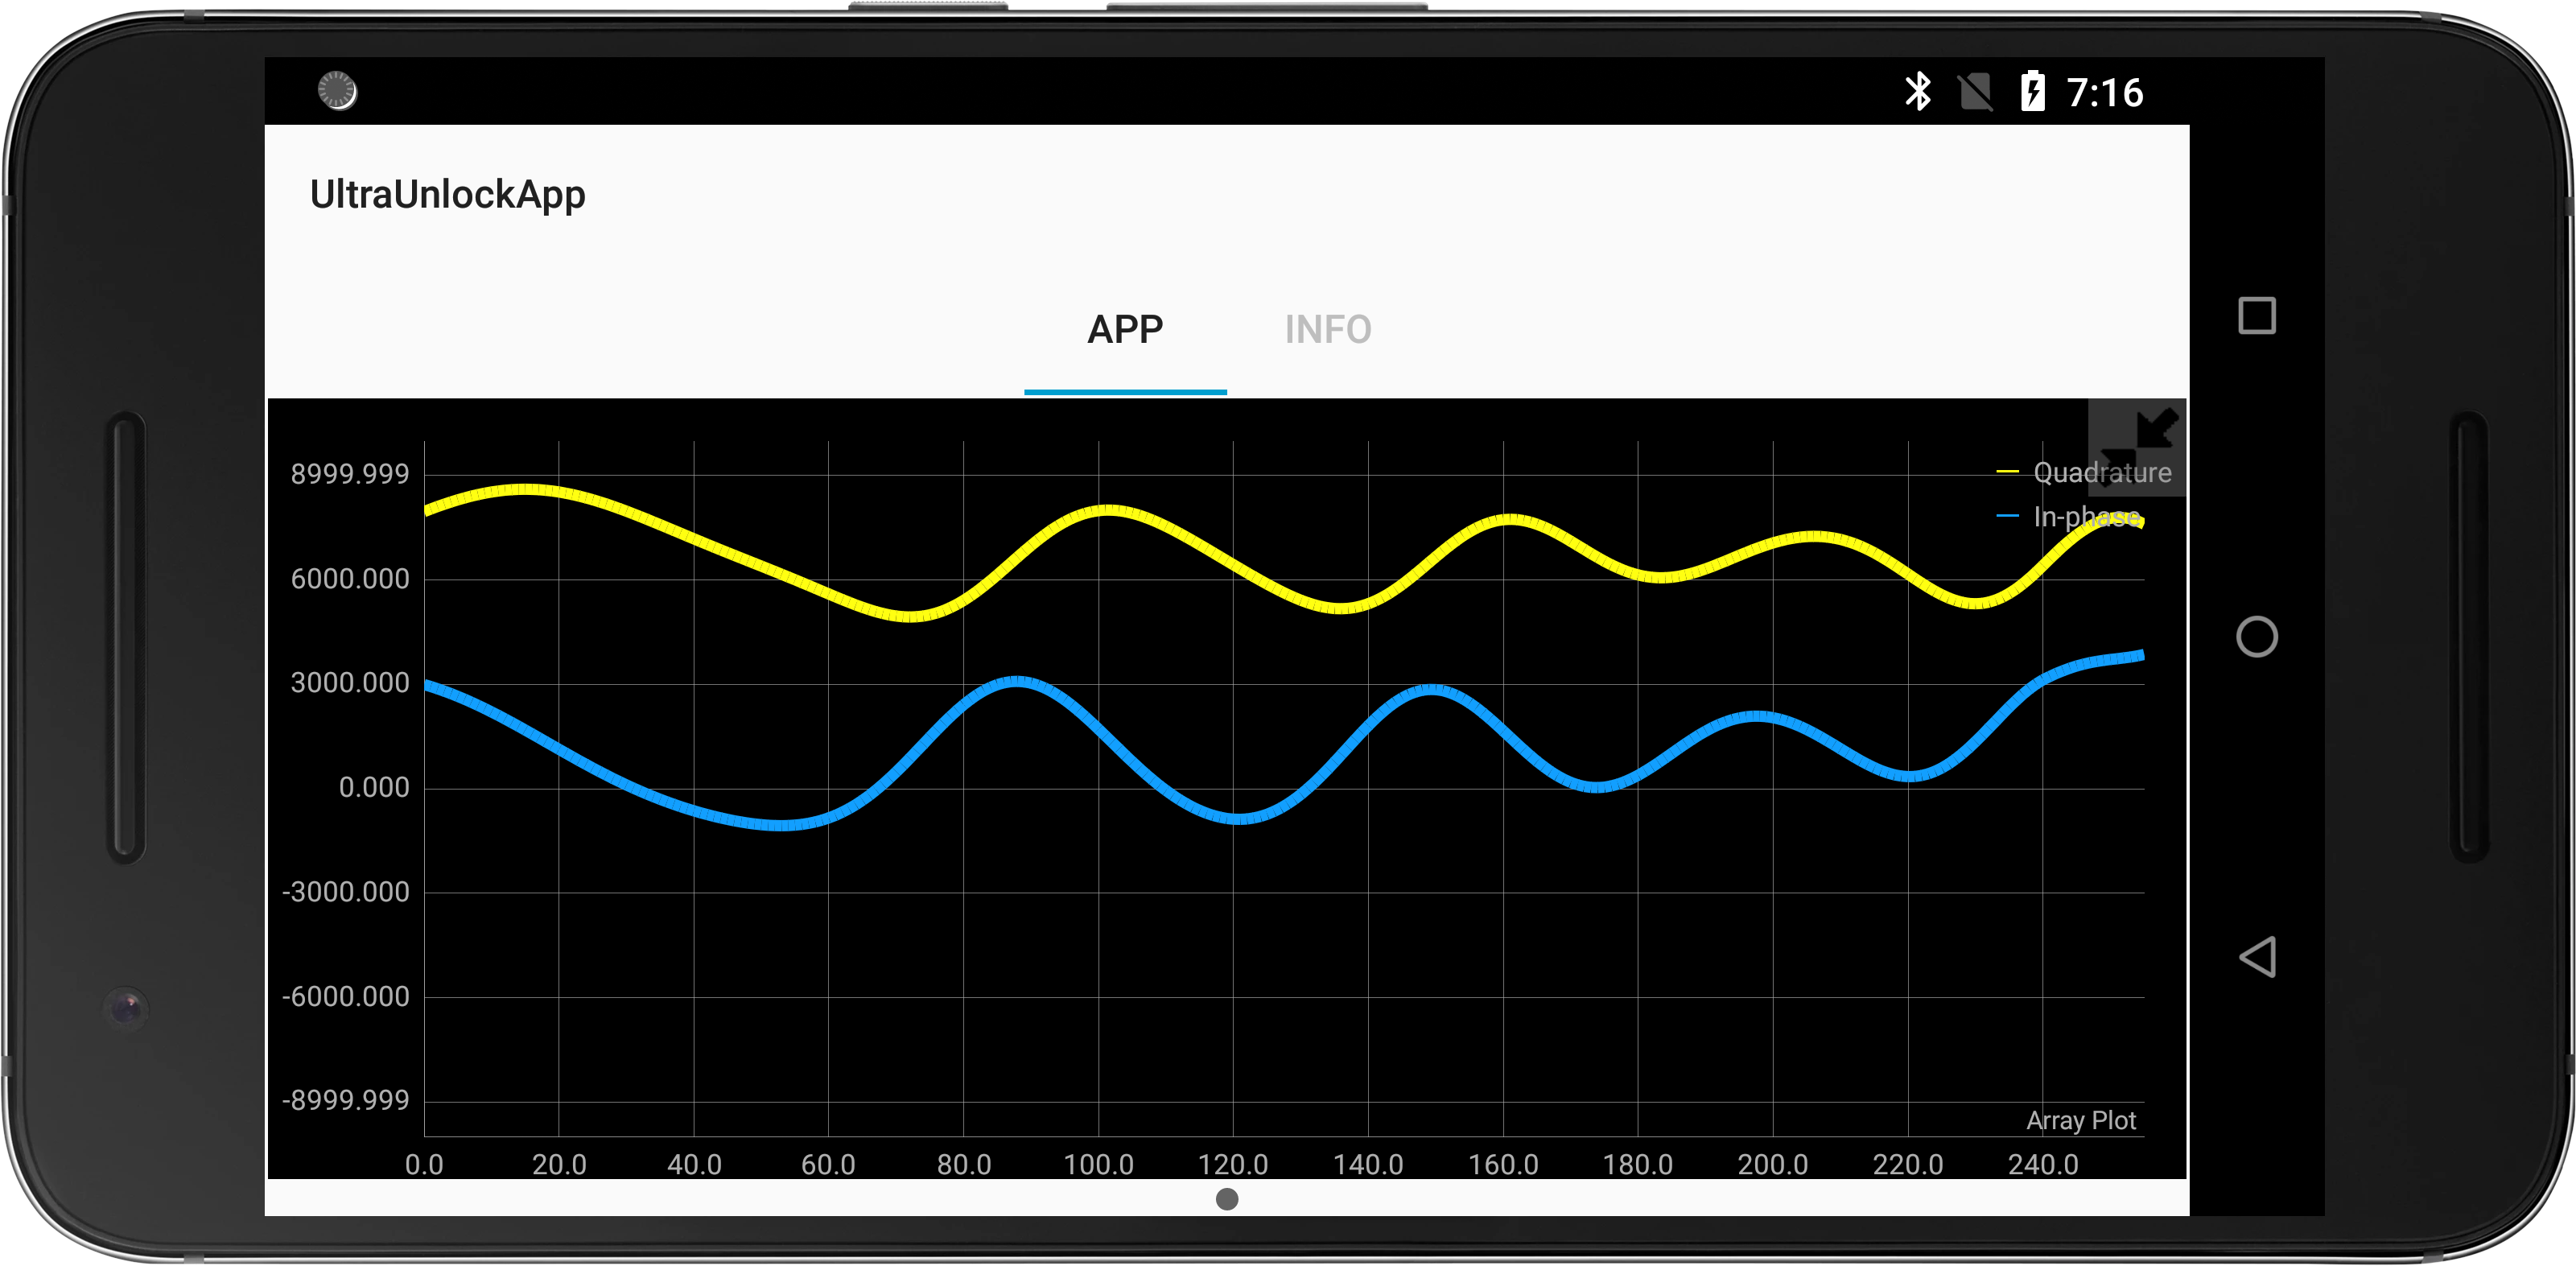
\includegraphics[width=\linewidth]{realiqdata1}
		\subcaption{One Hand Moving Towards the Phone}
		\vspace{.1in}
		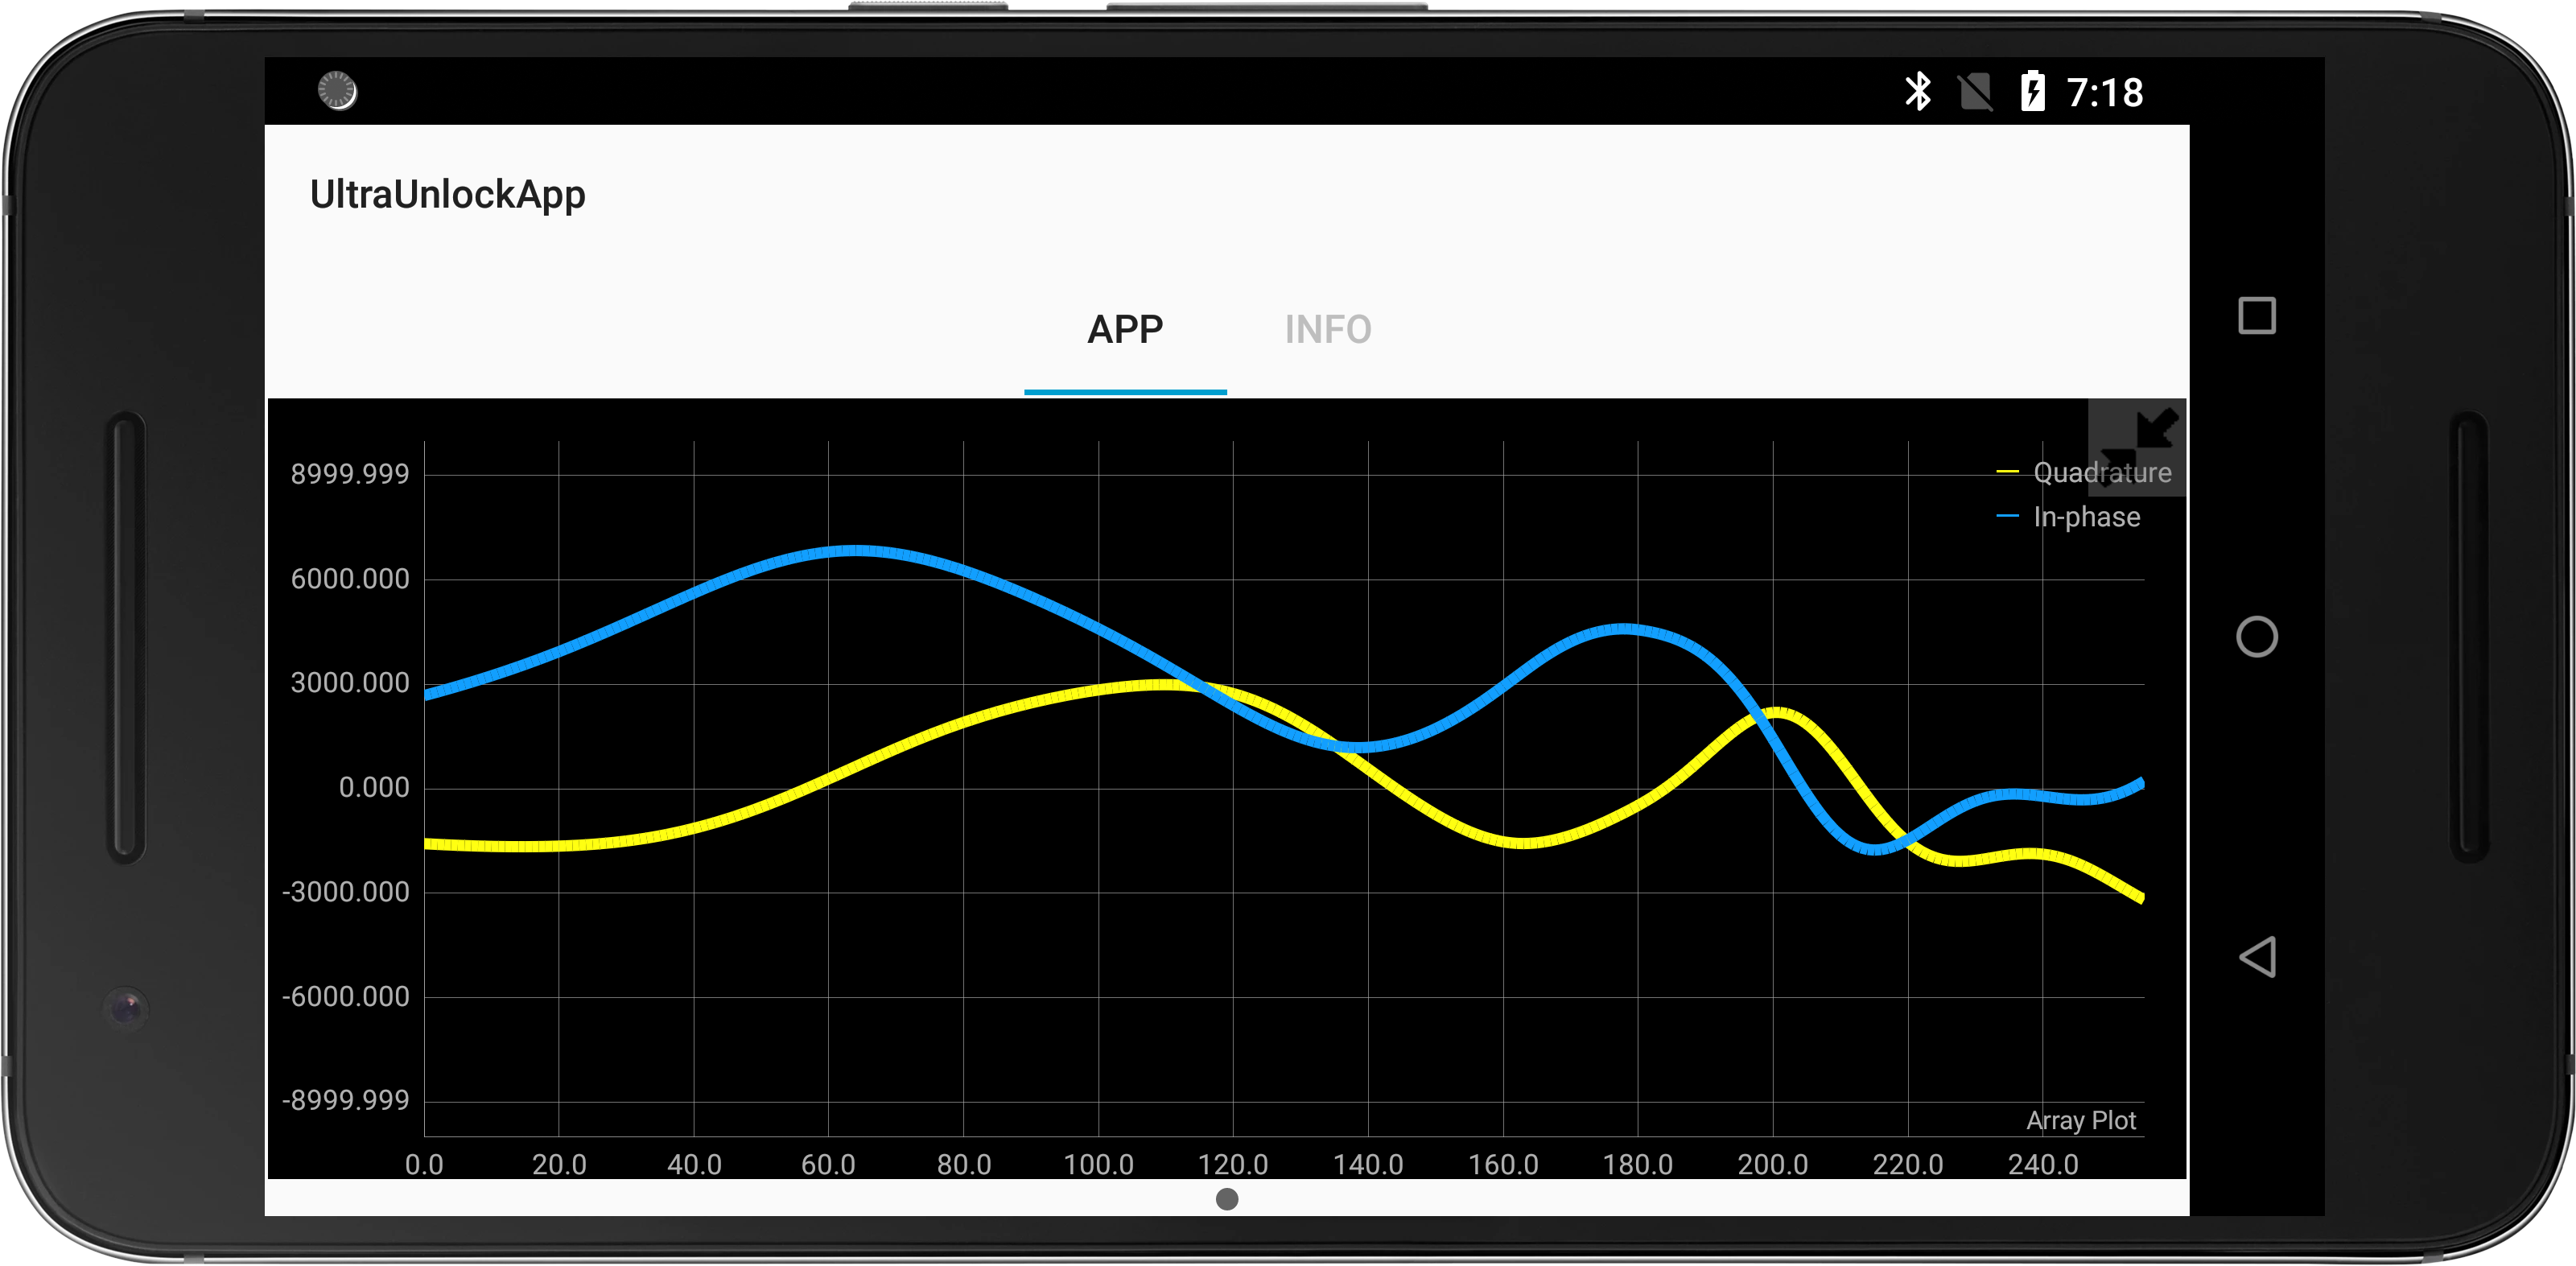
\includegraphics[width=\linewidth]{realiqdata2}
		\subcaption{Open-Close Gesture}
	\end{minipage}
	\caption{Screenshots of the UltraUnlockApp}	
	\label{fig:realIQ}
\end{figure}

\begin{figure}[!h]
	\centering
	\includegraphics[width=.8\linewidth]{androidiqdata1}
	\begin{minipage}{.4\linewidth}
		\includegraphics[width=\linewidth]{androidiqdata2}
	\end{minipage}
	\hfil
	\begin{minipage}{.5\linewidth}
		\includegraphics[width=\linewidth]{androidiqdata3}
		\includegraphics[width=\linewidth]{androidiqdata4}
	\end{minipage}
	\caption[I/Q Components Collected by UltraUnlockApp]{I/Q Components from Different View Angles. The hand first move dowards towards the smartphone, then move upwards.}
	\label{fig:androidiqdata}
\end{figure}

Figure~\ref{fig:androidiqdata} shows the I/Q data collected when the user moves the hand down and up. The phase of of the I/Q data inverses at 0.24 second, which indicates the direction change of the hand movement. Moreover, we noticed that there are 4 gull peaks and valleys before the hand change the direction. Combining with the fact that the wavelength of the signal is 1.72 cm, we know that the path changes $1.72 \times 4 = 6.88$ cm. In other words, in 0.2 second, the user moves one hand towards the smartphone by 3.44 cm. Note that this distance is calculated based on the assumption that the user hand moves in one dimension. However, in reality, user hands moves in 3D. Fortunately, smartphones nowadays are usually equipped with more than two speakers and more than two microphones, which enable {\uu} to locate user hands in 3D. Due to time limit, the current {\uu}App does not have this feature yet. In future work, we will implement this feature, as more dimensions of features will also increase the accuracy of user authentication.

\begin{figure}[h]
	\centering
	\begin{minipage}{.6\linewidth}
		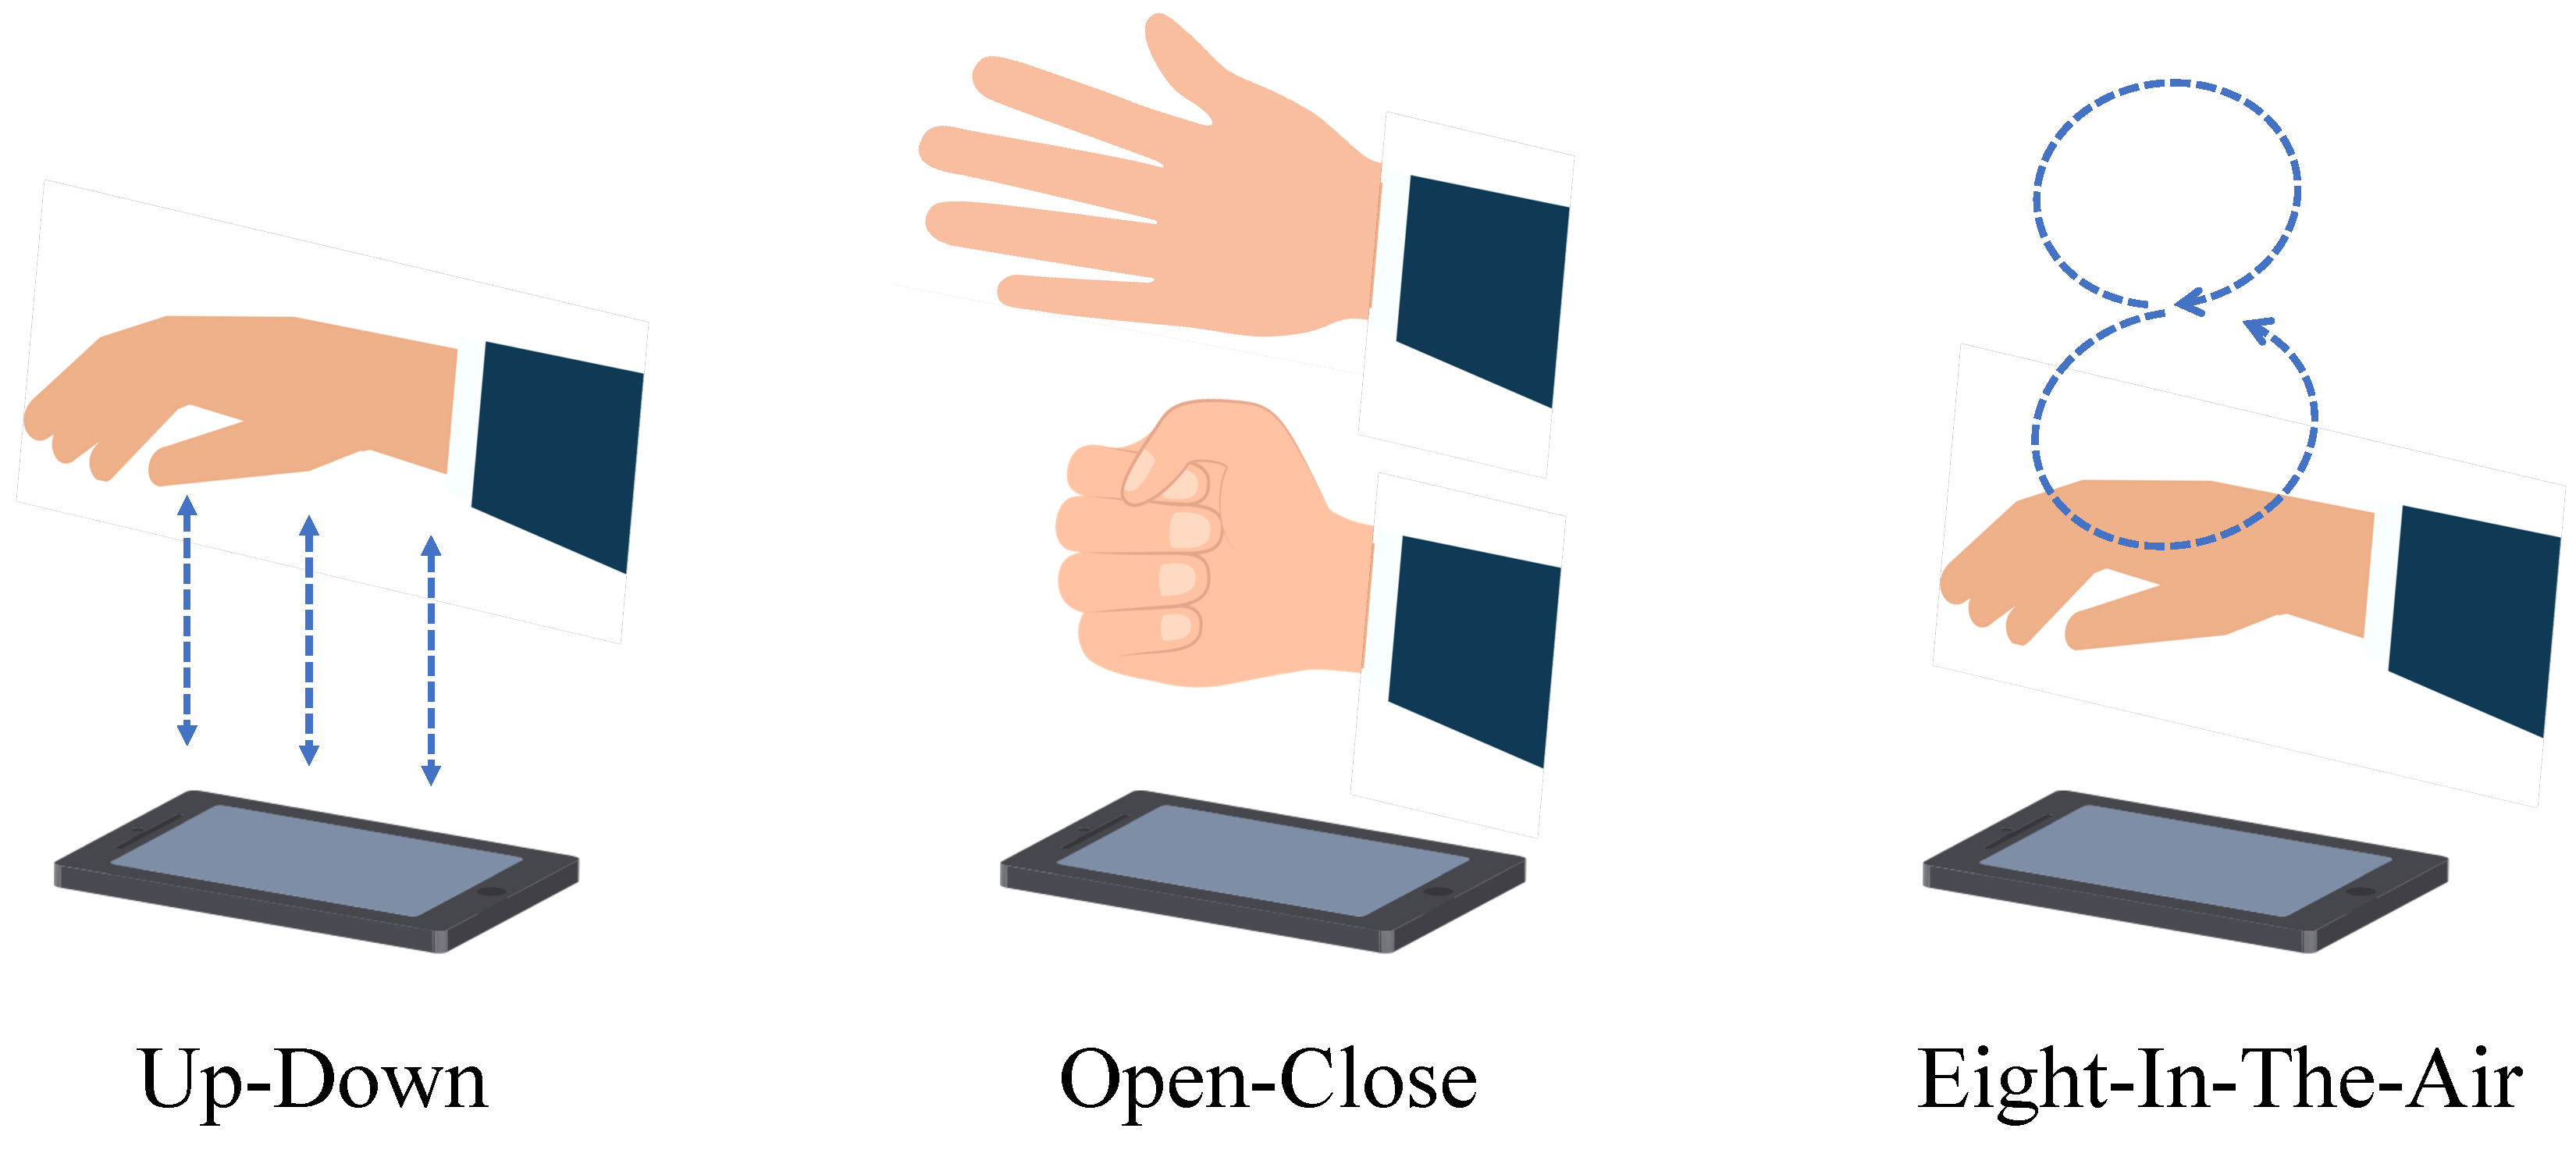
\includegraphics[width=\linewidth]{gestures}
	\end{minipage}
	\caption{Gestures tested in {\uu}.}	
	\label{fig:gestures}
\end{figure}


Our current machine learning modal only have two dimensions of features: the amplitude and the phase calculated from I/Q data. We tested our {\uu} system on 6 people and 3 gestures. Each user is asked to perform the same gestures for 20 times where we use half of them to train the LSTM network and the other half to test the model. The three gestures are: up-down, open-close, and drawing ``8'' in the air as shown in Figure~\ref{fig:gestures}. The 6 people are 3 females and 3 males aging 20-30. 


\begin{figure}[!h]
	\centering
	\begin{minipage}{.35\linewidth}
		\includegraphics[width=\linewidth]{gestureCFM}
		\vspace{.05in}
	\end{minipage}
	
	\centering
	%	\resizebox{\linewidth}{!}{
	\begin{tabular}{lr}
		\toprule
		Accuracy: 90.89\% & \hspace{-.55in} Error Rate: 9.11\% \\
		Precision: 92.04\% & \hspace{-.55in} True Positive Rate (Sensitivity/Recall): 91.00\% \\
		$F_1$ Score: 0.915 & \hspace{-.55in} True Negative Rate (Specificity): 95.10\% \\
		False Negative Rate: 9.00\%  & \hspace{-.55in} False Positive Rate: 4.90\% \\
		\bottomrule
	\end{tabular}
	\caption{The Confusion Matrix of the Gesture Classification Result.
	}
	\label{fig:gestureCFM}
\end{figure}

\begin{figure}[!h]
	\centering
	\begin{minipage}{.45\linewidth}
		\includegraphics[width=\linewidth]{userCFM}
		\vspace{.05in}
	\end{minipage}
	
	\centering
	%	\resizebox{\linewidth}{!}{
	\begin{tabular}{lr}
		\toprule
		Accuracy: 78.47\% & \hspace{-.55in} Error Rate: 21.53\% \\
		Precision: 77.74\% & \hspace{-.55in} True Positive Rate (Sensitivity/Recall): 77.69\% \\
		$F_1$ Score: 0.775 & \hspace{-.55in} True Negative Rate (Specificity): 95.68\% \\
		False Negative Rate: 22.31\%  & \hspace{-.55in} False Positive Rate: 4.32\% \\
		\bottomrule
	\end{tabular}
	\caption{The Confusion Matrix of the User Classification Result.
	}
	\label{fig:userCFM}
\end{figure}

The classification results of 3 gestures are shown in Figure~\ref{fig:gestureCFM}. The average accuracy is 90.89\% and the up-down gesture has the least false negative rate. The classification results of user identification is shown in Figure~\ref{fig:userCFM}, where the average accuracy is 78.47\%.  Note that the true negative rate (specificity) is 95.68\% and the false positive rate is 4.32\%, which means there is a higher chance that a legitimate user would be rejected than the chance that an attacker get accepted by the phone. Though such setting will provide more security to the smartphone, the overall accuracy is not satisfactory. There are at least three ways to further increase it, and we leave it for future work:
\begin{itemize}
	\item Utilizing more speakers and microphones. In this chapter, we only utilizing one microphone and one speaker on the smartphone. However, most smartphones nowadays support stereo audio, which means the device is equipped with at least a pair of microphones and a pair of speakers. If all sensors and transmitters are adopted, we will increase the signal channel from $1\times1$ to $2 \times2$. If doing so, {\uu} will be able to localize the hand in three dimensions and the feature vectors will increase from 2 to 8. Intuitively, the performance of the classification model will be improved with more features. However, there would also be many challenges to achieve the upgrades. For example, we need to propose effective and efficient algorithms to deal with the interference caused by the simultaneous signals.
	
	\item Using multiple-frequency signals as the carrier instead of single-frequency signals. Current {\uu} system suffers from the multipath effect. Ideally, when there is no hand movement, the I/Q data remain the same. However, signals received from different paths can be regarded as signals reflected by a moving hand, which causes the I/Q data being changed too. To mitigate the multipath effect, we could use signals with multiple frequencies as the carrier. Since those signals have different frequency and thus have different wavelength, they can differentiate between multiple stable paths and one varying path. The challenge is how to select those frequencies and how to set corresponding parameters for the CIC filters.
	
	\item Extracting more information from I/Q data instead of directly feeding them to LSTM networks. In this chapter, we feed the raw I/Q data to the machine learning model for classification. However, we could extract more information from them. With the aforementioned two improvement methods implemented, I/Q data can be used to reconstruct the hand trajectories in three dimensions. We can use the trajectories for user classification. Moreover, we could also extract time and frequency features from the I/Q data. Some commonly used temporal features include mean, min, max, RMS, ZCR, skewness, kurtosis, and peak cound. Some commonly used frequency features include spectral centroid, spectral spread,  spectral skewness,  spectral kurtosis,  spectral flatness, spectral irregularity, spectral entropy, spectral rolloff,	spectral brightness, 
	spectral RMS, and  spectral roughness. All these features can be implemented and tested to achieve higher accuracy. In addition, {\uu} now treats the hand and the fingers as an integrated part, reconstructing the gestures from hand level to finger level may improve the gesture recognition and user authentication performance.
	
	\item Implementing the system fully on smartphones. The current {\uu}App only serves as a data collection app, the training and predicting procedures are done in a MacBook Pro with 2.6 GHz 6-Core Intel Core i7 and 16 GB 2400 MHz DDR4. In future work, we will move this classification part to smartphones and evaluate the latency.
	
	
	\item Evaluating the performance of {\uu} under different settings. Many factors may have impact on the classification result. In the current experiments, we just showed the volunteers how to perform hand movements in the air. But we didn't restrict the users to perform the gestures in certain spaces. The volunteers were free to choose their own speed to draw the gestures and the size of the gestures is flexible too. In future work, we plan to test the influence of such factors. Moreover, current experiments are conducted in a relatively stable environment. There are no other moving objects within 1 meter of the testing smartphone. How to remove the noises from background movements is another challenge to overcome.
	
	
	\item Recruiting more volunteers and testing more gestures. In this chapter, {\uu} is tested over a very limited dataset. This is because of the limited time and the difficulties of recruiting volunteers during the pandemic. To popularize this new authentication method, a lot more volunteers and gestures are required. 
	
\end{itemize}


%========================================
%                            Section                             
%======================================== 	 
\section{Conclusion}
In this chapter, we demonstrated how to use I/Q data to represent hand movements and show the potential of using the I/Q data for smartphone authentication. Experiments showed that the proposed {\uu} system can achieve gesture recognition with accuracy of 90.8\% and user identification with accuracy of 78.47\%. This {\uu} system is till at its early stage and we pointed out six directions to improve it in future work.